\subsection{Testing Data Distribution Analysis}

\textbf{Why Ensure Balanced Testing Data?}
\begin{itemize}
	\item Prevents bias toward majority classes.
	\item Ensures fair evaluation across all sleep stages.
	\item Enhances generalization reliability.
\end{itemize}

The figure below shows the normalized class distribution during testing, confirming balance and the absence of class imbalance.

\begin{figure}[H]
	\centering
	\includegraphics[width=0.8\textwidth]{img/paper3/Analysis Plots/sample_distribution_plot_pdf.png}
	\caption{Balanced class distribution across the test set.}
\end{figure}

\subsection{Model Performance: Accuracy and Loss Trends}

Figures below illustrate the model's training vs testing accuracy and loss progression over epochs.

\begin{figure}[H]
	\centering
	\includegraphics[width=0.8\textwidth]{img/paper3/Analysis Plots/accuracy_plot.png}
	\caption{Accuracy Curve: Training vs Testing.}
\end{figure}

\begin{figure}[H]
	\centering
	\includegraphics[width=0.8\textwidth]{img/paper3/Analysis Plots/loss_plot.png}
	\caption{Loss Curve: Training vs Testing.}
\end{figure}

\subsection{Model Evaluation: Confusion Matrix and Evolution Metrics}

To evaluate classification performance, we compute the confusion matrix and derive the following metrics:

\[
\text{Precision} = \frac{TP}{TP + FP}, \quad
\text{Recall} = \frac{TP}{TP + FN}, \quad
\text{F1-Score} = \frac{2 \cdot \text{Precision} \cdot \text{Recall}}{\text{Precision} + \text{Recall}}
\]

Additionally, we compute the evolution matrix \( E \) that captures the transition probabilities between predicted and true classes:

\[
E(i, j) = \frac{C(i, j)}{\sum_{k} C(i, k)}
\]

Where \( C(i, j) \) is the confusion matrix count for true class \( i \) predicted as class \( j \).

\begin{figure}[H]
	\centering
	\includegraphics[width=0.8\textwidth]{img/paper3/Analysis Plots/confusion_matrix_samples.png}
	\caption{Confusion Matrix showing model performance across sleep stages.}
\end{figure}

\subsection{Gradient Analysis Across Training}

Model training stability was assessed via gradient trends:

\begin{itemize}
	\item \textbf{Epochs 0–5:} High loss, gradual accuracy increase.
	\item \textbf{Epochs 5–15:} Stable gradient flow and decreasing loss.
	\item \textbf{Epochs 15–20:} Accuracy plateaus, no overfitting.
\end{itemize}

\textbf{Conclusion:} Training remained stable with no vanishing/exploding gradients.

\begin{figure}[H]
	\centering
	\includegraphics[width=0.8\textwidth]{img/paper3/Analysis Plots/3d_gradient.png}
	\caption{Gradient 3D Surface: Training vs Validation Metrics.}
\end{figure}

\subsection{Performance Metrics: Class-wise Scores}

Key metrics computed per class to understand classification effectiveness:

\begin{figure}[H]
	\centering
	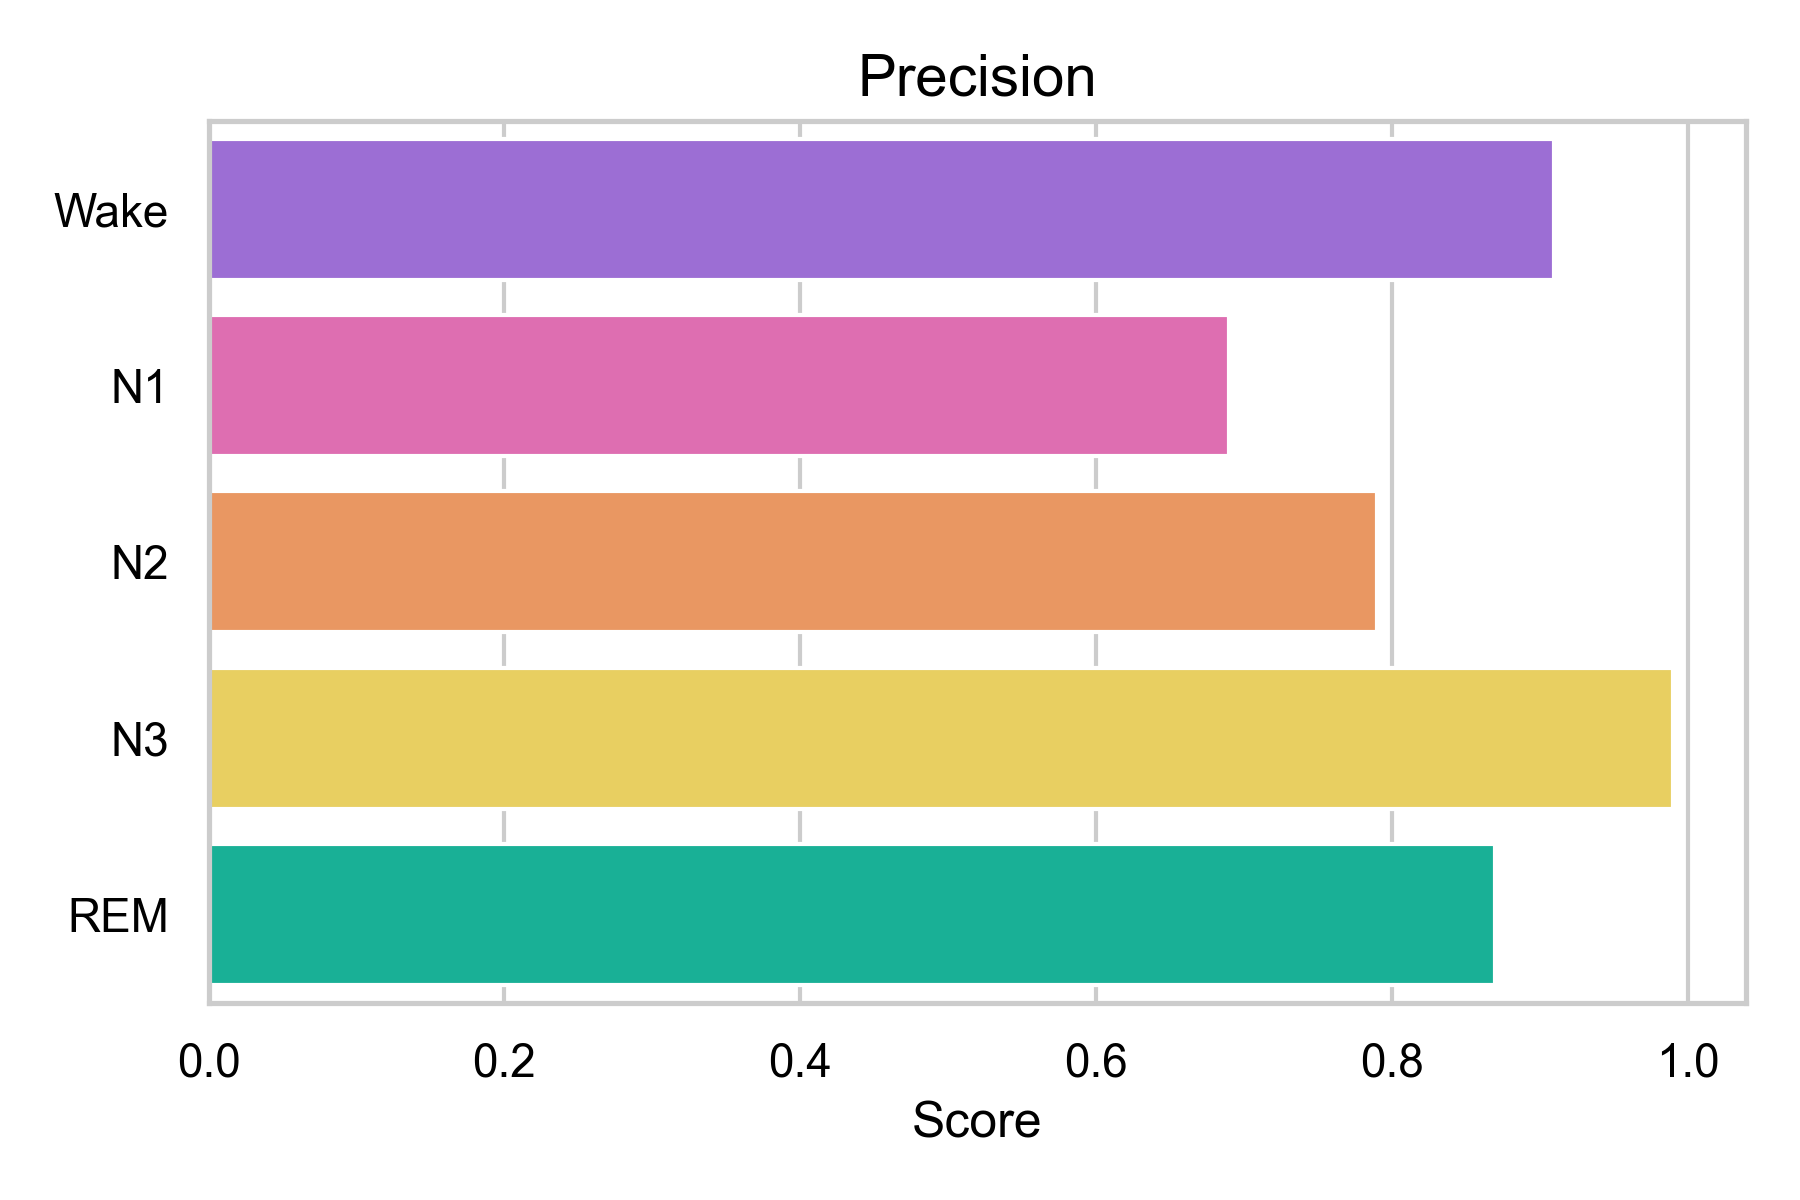
\includegraphics[width=0.8\textwidth]{img/paper3/Analysis Plots/precision_plot.png}
	\caption{Precision Scores per Class.}
\end{figure}

\begin{figure}[H]
	\centering
	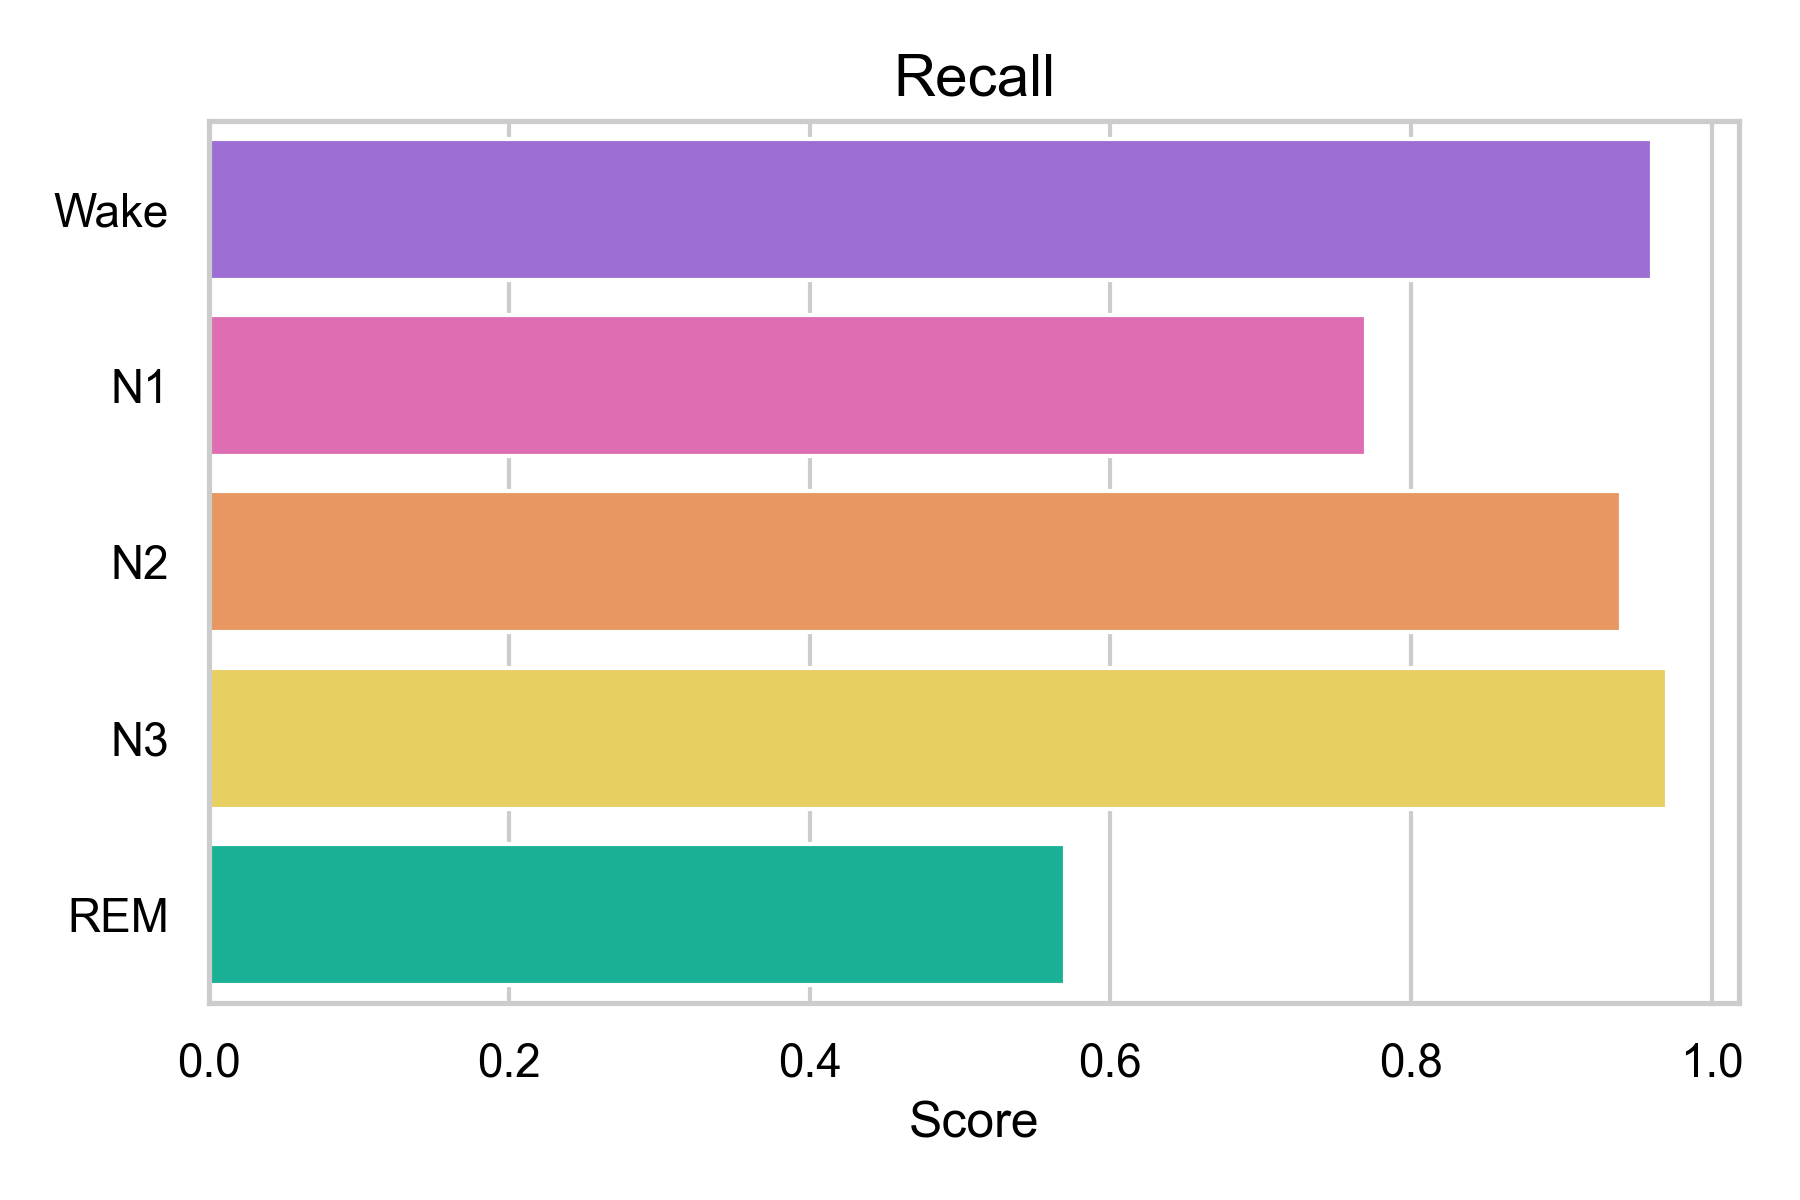
\includegraphics[width=0.8\textwidth]{img/paper3/Analysis Plots/recall_plot.png}
	\caption{Recall Scores per Class.}
\end{figure}

\begin{figure}[H]
	\centering
	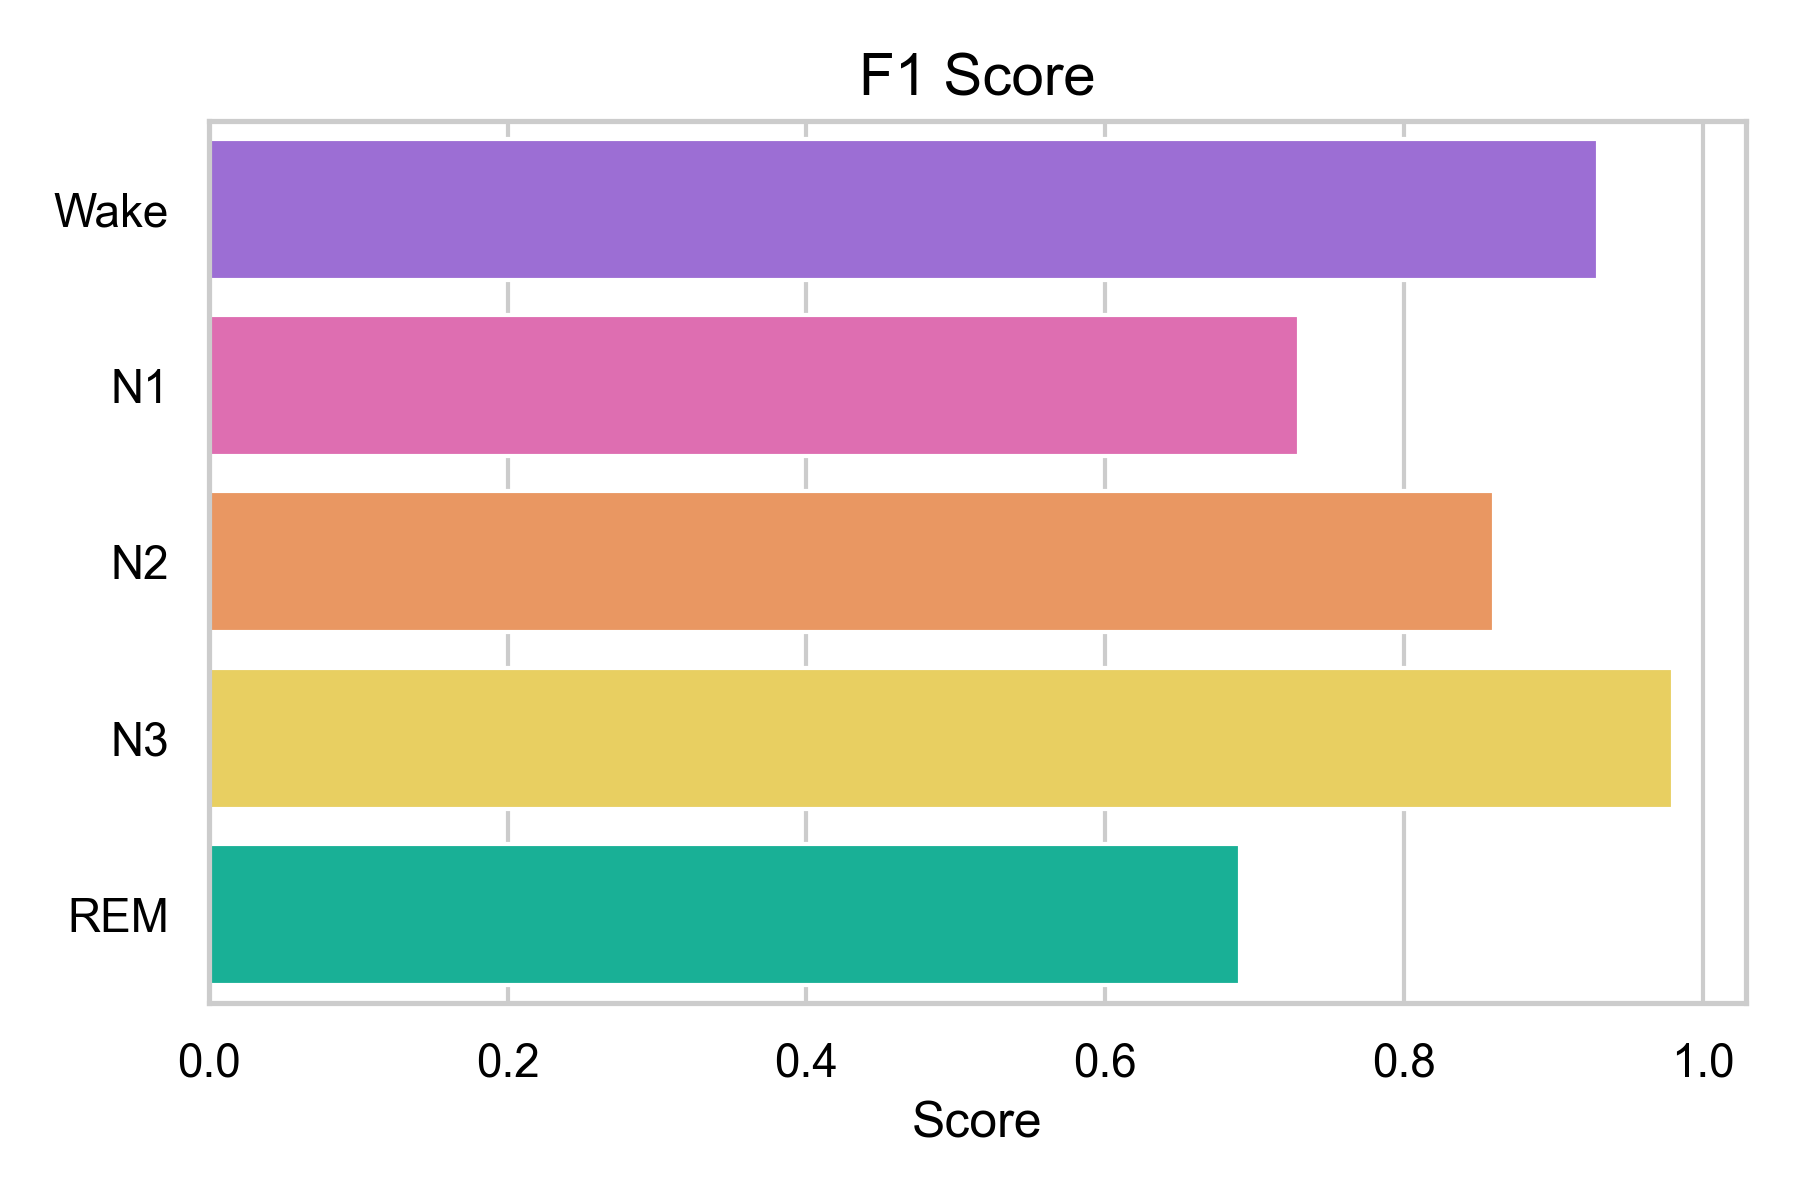
\includegraphics[width=0.8\textwidth]{img/paper3/Analysis Plots/f1_score_plot.png}
	\caption{F1 Scores per Class.}
\end{figure}

\subsection{Feature Importance Analysis using LIME}

We used LIME to interpret feature contributions. The results highlight:

\begin{itemize}
	\item \textbf{Most influential:} EMG submental, EEG Pz-Oz
	\item \textbf{Least influential:} EOG horizontal
\end{itemize}

This helps refine feature selection and optimize performance.

\begin{figure}[H]
	\centering
	\includegraphics[width=0.8\textwidth]{img/paper3/Analysis Plots/feature_importance_chanels_analysis.png}
	\caption{Feature Importance Analysis for 4 Channels using LIME.}
\end{figure}
